% Options for packages loaded elsewhere
\PassOptionsToPackage{unicode}{hyperref}
\PassOptionsToPackage{hyphens}{url}
\PassOptionsToPackage{dvipsnames,svgnames,x11names}{xcolor}
%
\documentclass[
  conference]{IEEEtran}

\usepackage{amsmath,amssymb}
\usepackage{lmodern}
\usepackage{iftex}
\ifPDFTeX
  \usepackage[T1]{fontenc}
  \usepackage[utf8]{inputenc}
  \usepackage{textcomp} % provide euro and other symbols
\else % if luatex or xetex
  \usepackage{unicode-math}
  \defaultfontfeatures{Scale=MatchLowercase}
  \defaultfontfeatures[\rmfamily]{Ligatures=TeX,Scale=1}
\fi
% Use upquote if available, for straight quotes in verbatim environments
\IfFileExists{upquote.sty}{\usepackage{upquote}}{}
\IfFileExists{microtype.sty}{% use microtype if available
  \usepackage[]{microtype}
  \UseMicrotypeSet[protrusion]{basicmath} % disable protrusion for tt fonts
}{}
\makeatletter
\@ifundefined{KOMAClassName}{% if non-KOMA class
  \IfFileExists{parskip.sty}{%
    \usepackage{parskip}
  }{% else
    \setlength{\parindent}{0pt}
    \setlength{\parskip}{6pt plus 2pt minus 1pt}}
}{% if KOMA class
  \KOMAoptions{parskip=half}}
\makeatother
\usepackage{xcolor}
\setlength{\emergencystretch}{3em} % prevent overfull lines
\setcounter{secnumdepth}{5}
% Make \paragraph and \subparagraph free-standing
\ifx\paragraph\undefined\else
  \let\oldparagraph\paragraph
  \renewcommand{\paragraph}[1]{\oldparagraph{#1}\mbox{}}
\fi
\ifx\subparagraph\undefined\else
  \let\oldsubparagraph\subparagraph
  \renewcommand{\subparagraph}[1]{\oldsubparagraph{#1}\mbox{}}
\fi


\providecommand{\tightlist}{%
  \setlength{\itemsep}{0pt}\setlength{\parskip}{0pt}}\usepackage{longtable,booktabs,array}
\usepackage{calc} % for calculating minipage widths
% Correct order of tables after \paragraph or \subparagraph
\usepackage{etoolbox}
\makeatletter
\patchcmd\longtable{\par}{\if@noskipsec\mbox{}\fi\par}{}{}
\makeatother
% Allow footnotes in longtable head/foot
\IfFileExists{footnotehyper.sty}{\usepackage{footnotehyper}}{\usepackage{footnote}}
\makesavenoteenv{longtable}
\usepackage{graphicx}
\makeatletter
\def\maxwidth{\ifdim\Gin@nat@width>\linewidth\linewidth\else\Gin@nat@width\fi}
\def\maxheight{\ifdim\Gin@nat@height>\textheight\textheight\else\Gin@nat@height\fi}
\makeatother
% Scale images if necessary, so that they will not overflow the page
% margins by default, and it is still possible to overwrite the defaults
% using explicit options in \includegraphics[width, height, ...]{}
\setkeys{Gin}{width=\maxwidth,height=\maxheight,keepaspectratio}
% Set default figure placement to htbp
\makeatletter
\def\fps@figure{htbp}
\makeatother
\newlength{\cslhangindent}
\setlength{\cslhangindent}{1.5em}
\newlength{\csllabelwidth}
\setlength{\csllabelwidth}{3em}
\newlength{\cslentryspacingunit} % times entry-spacing
\setlength{\cslentryspacingunit}{\parskip}
\newenvironment{CSLReferences}[2] % #1 hanging-ident, #2 entry spacing
 {% don't indent paragraphs
  \setlength{\parindent}{0pt}
  % turn on hanging indent if param 1 is 1
  \ifodd #1
  \let\oldpar\par
  \def\par{\hangindent=\cslhangindent\oldpar}
  \fi
  % set entry spacing
  \setlength{\parskip}{#2\cslentryspacingunit}
 }%
 {}
\usepackage{calc}
\newcommand{\CSLBlock}[1]{#1\hfill\break}
\newcommand{\CSLLeftMargin}[1]{\parbox[t]{\csllabelwidth}{#1}}
\newcommand{\CSLRightInline}[1]{\parbox[t]{\linewidth - \csllabelwidth}{#1}\break}
\newcommand{\CSLIndent}[1]{\hspace{\cslhangindent}#1}

\usepackage{cite}
\usepackage{amsmath,amssymb,amsfonts}
\usepackage{algorithm}% http://ctan.org/pkg/algorithms
\usepackage{algpseudocode}% http://ctan.org/pkg/algorithmicx
\usepackage{graphicx}
\usepackage{textcomp}
\usepackage{xcolor}
\usepackage{placeins}
\def\BibTeX{{\rm B\kern-.05em{\sc i\kern-.025em b}\kern-.08em
    T\kern-.1667em\lower.7ex\hbox{E}\kern-.125emX}}
\makeatletter
\makeatother
\makeatletter
\makeatother
\makeatletter
\@ifpackageloaded{caption}{}{\usepackage{caption}}
\AtBeginDocument{%
\ifdefined\contentsname
  \renewcommand*\contentsname{Table of contents}
\else
  \newcommand\contentsname{Table of contents}
\fi
\ifdefined\listfigurename
  \renewcommand*\listfigurename{List of Figures}
\else
  \newcommand\listfigurename{List of Figures}
\fi
\ifdefined\listtablename
  \renewcommand*\listtablename{List of Tables}
\else
  \newcommand\listtablename{List of Tables}
\fi
\ifdefined\figurename
  \renewcommand*\figurename{Figure}
\else
  \newcommand\figurename{Figure}
\fi
\ifdefined\tablename
  \renewcommand*\tablename{Table}
\else
  \newcommand\tablename{Table}
\fi
}
\@ifpackageloaded{float}{}{\usepackage{float}}
\floatstyle{ruled}
\@ifundefined{c@chapter}{\newfloat{codelisting}{h}{lop}}{\newfloat{codelisting}{h}{lop}[chapter]}
\floatname{codelisting}{Listing}
\newcommand*\listoflistings{\listof{codelisting}{List of Listings}}
\makeatother
\makeatletter
\@ifpackageloaded{caption}{}{\usepackage{caption}}
\@ifpackageloaded{subcaption}{}{\usepackage{subcaption}}
\makeatother
\makeatletter
\@ifpackageloaded{tcolorbox}{}{\usepackage[many]{tcolorbox}}
\makeatother
\makeatletter
\@ifundefined{shadecolor}{\definecolor{shadecolor}{rgb}{.97, .97, .97}}
\makeatother
\makeatletter
\makeatother
\ifLuaTeX
  \usepackage{selnolig}  % disable illegal ligatures
\fi
\IfFileExists{bookmark.sty}{\usepackage{bookmark}}{\usepackage{hyperref}}
\IfFileExists{xurl.sty}{\usepackage{xurl}}{} % add URL line breaks if available
\urlstyle{same} % disable monospaced font for URLs
\hypersetup{
  pdftitle={Endogenous Macrodynamics in Algorithmic Recourse},
  colorlinks=true,
  linkcolor={blue},
  filecolor={Maroon},
  citecolor={Blue},
  urlcolor={Blue},
  pdfcreator={LaTeX via pandoc}}

\title{Endogenous Macrodynamics in Algorithmic Recourse}
\author{}
\date{}

\begin{document}
\maketitle
\begin{abstract}
Existing work on Counterfactual Explanations (CE) and Algorithmic
Recourse (AR) has largely been limited to the static setting: given some
classifier we are interested in finding close, actionable, realistic,
sparse, diverse and ideally causally founded counterfactuals. The
ability of CE to handle dynamics like data and model drift remains a
largely unexplored research challenge at this point. Only one recent
work considers the implications of exogenous domain and model shifts.
This project instead focuses on endogenous dynamics, that is shifts that
occur when AR is actually implemented by a proportion of individuals.
Early findings suggest that the involved shifts may be large with
important implications on the validity of AR and the overall
characteristics of the sample population.
\end{abstract}
\ifdefined\Shaded\renewenvironment{Shaded}{\begin{tcolorbox}[interior hidden, borderline west={3pt}{0pt}{shadecolor}, enhanced, boxrule=0pt, frame hidden, sharp corners, breakable]}{\end{tcolorbox}}\fi

\hypertarget{sec-intro}{%
\section{Introduction}\label{sec-intro}}

Recent advances in Artificial Intelligence (AI) have propelled its
adoption in scientific domains outside of Computer Science including
Healthcare, Bioinformatics, Genetics and the Social Sciences. While this
has in many cases brought benefits in terms of efficiency,
state-of-the-art models like Deep Neural Networks (DNN) have also given
rise a new type of principal-agent problem in the context of data-driven
decision-making. It involves a group of \textbf{principals} - i.e.~human
stakeholders - that fail to understand the behaviour of their
\textbf{agent} - i.e.~the model used for automated decision-making
\protect\hyperlink{ref-borch2022machine}{{[}1{]}}.

Models or algorithms that fall into this category are typically referred
to \textbf{black-box} models. Despite their shortcomings, black-box
models have grown in popularity in recent years and have at times
created undesirable societal outcomes
\protect\hyperlink{ref-o2016weapons}{{[}2{]}}. The scientific community
has tackled this issue from two different angles: while some have
appealed for a strict focus on inherently iterpretable models
\protect\hyperlink{ref-rudin2019stop}{{[}3{]}}, others have investigated
different ways to explain the behaviour of black-box models. These two
sub-domains can be broadly referred to as \textbf{interpretable AI} and
\textbf{explainable AI} (XAI), respectively.

Among the approaches to XAI that have recently grown in popularity are
\textbf{Counterfactual Explanations} (CE). They explain how inputs into
a model need to change for it to produce different outputs.
Counterfactual Explanations that involve realistic and actionable
changes can be used for the purpose of \textbf{Algorithmic Recourse}
(AR) to help individuals who face adverse outcomes. An example relevant
to the Social Sciences is consumer credit: in this context AR can be
used to guide individuals in improving their creditworthiness, should
they have previously been denied access to credit based on an automated
decision-making system. A meaningful recourse recommendation for a
denied applicant could be: \emph{``If your net savings rate had been
10\% of your monthly income instead of the actual 8\%, your application
would have been successful. See if you can temporarily cut down on
consumption.''} In the remainder of this paper we will use both
terminologies - recourse and counterfactual - interchangeably to refer
to situations where counterfactuals are generated with the intent to
provide individual recourse.

Existing work in this field has largely worked in a static setting:
various approaches have been proposed to generate counterfactuals for a
given individual that is subject to some pre-trained model. More recent
work has compared different approaches within this static setting
\protect\hyperlink{ref-pawelczyk2021carla}{{[}4{]}}. In this work we go
one step further and ask ourselves: what happens if recourse is provided
and implemented repeatedly? What types of dynamics are introduced and
how do different counterfactual generators compare in this context?

Figure~\ref{fig-poc} illustrates this idea for a binary problem
involving a probabilistic classifier and the counterfactual generator
proposed by \protect\hyperlink{ref-wachter2017counterfactual}{{[}5{]}}:
the implementation of AR for a subset of individuals leads to a domain
shift (b), which in turn triggers a model shift (c). As this game of
implementing AR and updating the classifier is repeated, the decision
boundary moves away from training samples that were originally in the
target class (d). We refer to these types of dynamics as
\textbf{endogenous} because they are induced by the implementation of
recourse itself.

\begin{figure}

{\centering 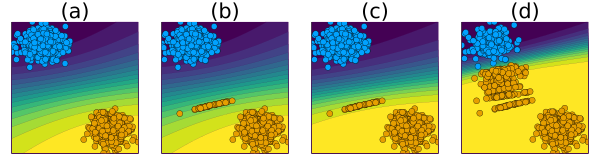
\includegraphics[width=0.45\textwidth,height=\textheight]{www/poc.png}

}

\caption{\label{fig-poc}Dynamics in Algorithmic Recourse: we have a
simple Bayesian model trained for binary classification (a); the
implementation of AR for a random subset of individuals leads to a
domain shift (b); as the classifier is retrained we observe a model
shift (c); as this process is repeated, the decision boundary moves away
from the target class (d).}

\end{figure}

We think that these types of endogenous dynamics may be problematic.
Firstly, model shifts may inadvertently change classification outcomes
for individuals who never received and implemented recourse. Secondly
and relatedly, we observe in Figure~\ref{fig-poc} that as the decision
boundary moves in the direction of the non-target class, counterfactual
paths become shorter: in the consumer credit example, individuals that
previously would have been denied credit based on their input features
are suddenly considered as creditworthy. Average default risk across all
borrowers can therefore be expected to increase. Conversely, lenders
that anticipate such dynamics may choose to deny credit to individuals
that have implemented AR, thereby compromising the validity of AR.

To the best of our knowledge this is the first work investigating
endogenous dynamics in AR. Our contributions to the state of knowledge
are two-fold. Firstly, we introduce an experimental framework extending
previous work by \protect\hyperlink{ref-pawelczyk2021carla}{{[}4{]}},
which allows for benchmarking different counterfactual generators in
terms of the endogenous domain and model shifts they introduce. To this
end we propose a number of novel evaluation metrics. Secondly, we use
this framework to provide the first in-depth analysis of endogenous
recourse dynamics induced by various popular counterfactual generators
including \protect\hyperlink{ref-wachter2017counterfactual}{{[}5{]}},
\protect\hyperlink{ref-joshi2019towards}{{[}6{]}},
\protect\hyperlink{ref-mothilal2020explaining}{{[}7{]}} and
\protect\hyperlink{ref-antoran2020getting}{{[}8{]}}.

We find that \ldots{}

The paper is structured as follows: Section~\ref{sec-related} places our
work in the broader context of related literature.
Section~\ref{sec-method} presents our methodology and data.
Section~\ref{sec-empirical} presents our empirical findings which are
then discussed in Section~\ref{sec-discussion}. We also point to some of
the limitations or our work as well as avenues for future research in
Section~\ref{sec-limit}. Finally, Section~\ref{sec-conclusion}
concludes.

\hypertarget{sec-related}{%
\section{Related Work}\label{sec-related}}

In this Section we provide a review of the relevant literature. First,
Section~\ref{sec-related-recourse} discusses the existing research
within the domain of counterfactual explanations and algorithmic
recourse. Then, Section~\ref{sec-related-shifts} presents some of the
previous work on the measurement of dataset and model shifts.

\hypertarget{sec-related-recourse}{%
\subsection{Algorithmic Recourse}\label{sec-related-recourse}}

A framework for Counterfactual Explanations was first proposed in 2017
by \protect\hyperlink{ref-wachter2017counterfactual}{{[}5{]}} and has
served as the baseline for most methodologies that have been proposed
since then. Let \(M: \mathcal{X} \mapsto \mathcal{Y}\) denote some
pre-trained model that maps from inputs \(X \in \mathcal{X}\) to outputs
\(Y \in \mathcal{Y}\). Then we are interested in minimizing the
complexity or effort \(H=h(x\prime)\) associated with moving an
individual \(x\) to a counterfactual state \(x\prime\) such that the
predicted outcome \(M(x\prime)\) corresponds to some target outcome
\(t\):

\begin{equation}\protect\hypertarget{eq-obj}{}{
\min_{x\prime \in \mathcal{x}} c(x\prime) \ \ \ \mbox{s. t.} \ \ \ M(x\prime) = t
}\label{eq-obj}\end{equation}

For implementation purposes, Equation~\ref{eq-obj} is typically
approximated through regularization:

\begin{equation}\protect\hypertarget{eq-solution}{}{
x\prime = \arg \min_{x\prime}  \ell(M(x\prime),t) + \lambda h(x\prime)
}\label{eq-solution}\end{equation}

In the baseline work and many subsequent approaches the complexity
function \(h: \mathcal{X} \mapsto \mathbb{R}\) is proxied by some
distance metric based on the simple intuition that large perturbations
of \(x\) are costly.

Many approaches for the generation of algorithmic recourse have been
described in the literature. An October 2020 survey by Karimi et
al.~layed out 60 algorithms that have been proposed since 2014
\protect\hyperlink{ref-karimi2020survey}{{[}9{]}}. Another survey
published around the same time by Verma et al.~described 29 algorithms
\protect\hyperlink{ref-verma2020counterfactual}{{[}10{]}}. Different
approaches vary primarily in terms of the objective functions they
impose, how they optimize said objective (from brute force through
gradient-based approaches to graph traversal algorithms), and how the
ensure that certain requirements for CE are met. Regarding the latter,
the literature has produced an extensive list of desiderata each
addressing different needs. To name but a few, we are interested in
generating counterfactuals that close
\protect\hyperlink{ref-wachter2017counterfactual}{{[}5{]}}, actionable
\protect\hyperlink{ref-ustun2019actionable}{{[}11{]}}, realistic
\protect\hyperlink{ref-schut2021generating}{{[}12{]}}, sparse, diverse
\protect\hyperlink{ref-mothilal2020explaining}{{[}7{]}} and if possible
causally founded
\protect\hyperlink{ref-karimi2021algorithmic}{{[}13{]}}.

Efforts so far have largely been directed at improving the quality of
counterfactual explanations within a static context: given some
pre-trained classifier \(M: \mathcal{X} \mapsto \mathcal{Y}\) we are
interested in generating one or multiple meaningful counterfactual
explanations for some individual characterized by \(x_i\). The ability
of counterfactual explanations to handle dynamics like data and model
shifts remains a largely unexplored research challenge at this point
\protect\hyperlink{ref-verma2020counterfactual}{{[}10{]}}. We have been
able to identify only one recent work that considers the implications of
\textbf{exogenous} domain and model shifts in the context of AR
\protect\hyperlink{ref-upadhyay2021towards}{{[}14{]}}. Exogenous shifts
are strictly of external origin. For example, they might stem from data
correction, temporal shifts or geospatial changes
\protect\hyperlink{ref-upadhyay2021towards}{{[}14{]}}. The authors of
\protect\hyperlink{ref-upadhyay2021towards}{{[}14{]}} propose framework
for algorithmic recourse (ROAR) that evidently improves robustness to
such exogenous shifts.

\hypertarget{sec-related-shifts}{%
\subsection{Domain and Model Shifts}\label{sec-related-shifts}}

Much attention has been paid to the detection of dataset shifts --
situations where the distribution of data changes over time. Rabanser et
al.~suggest a framework to detect data drift from a minimal number of
samples through the application of two-sample tests
\protect\hyperlink{ref-rabanser2019failing}{{[}15{]}}. This task is a
generalization of the anomaly detection problem for large datasets,
which aims to answer the question if two sets of samples could have been
generated from the same probability distribution. Numerous approaches to
anomaly detection have been summarized
\protect\hyperlink{ref-chandola2009anomaly}{{[}16{]}}. Another
well-established research topic is that of concept drift -- situations
where external variables influence the patterns between the input and
the output of a model
\protect\hyperlink{ref-widmer1996learning}{{[}17{]}}. For instance, Gama
et al.~offer a review of the adaptive learning techniques which can
handle concept drift \protect\hyperlink{ref-gama2014survey}{{[}18{]}}.
Less previous work is available on the related topic of model drift -
changes in model performance over time. Nelson et al.~review how
resistant different machine learning models are to the model drift
\protect\hyperlink{ref-nelson2015evaluating}{{[}19{]}}. Ackerman et
al.~offer a method to detect changes in model performance when ground
truth is not available
\protect\hyperlink{ref-ackerman2021machine}{{[}20{]}}.

In the context of algorithmic recourse, domain and model shifts were
first brought up by the authors behind ROAR
\protect\hyperlink{ref-upadhyay2021towards}{{[}14{]}}. In their work
they refer to model shifts as simply any perturbation \(\Delta\) to the
parameters of the model in question: \(M\). While this also sets the
baseline for our analysis here, it is worth noting that in
\protect\hyperlink{ref-upadhyay2021towards}{{[}14{]}} these
perturbations are mechanically introduced. In contrast we are interested
in quantifying model shifts that arise endogenously as part of a dynamic
recourse process. In addition to quantifying the magnitude of shifts
\(\Delta\), we aim to also analyse the characteristics of changes to the
model, such as the position of the decision boundary and the overall
decisiveness of the model. We have not been able to identify previous
work on this topic.

\hypertarget{sec-related-benchmark}{%
\subsection{Benchmarking Counterfactual
Generators}\label{sec-related-benchmark}}

Despite the large and growing number of approaches to counterfactual
search there have been surprisingly few benchmark studies that compare
different methodologies. This may be partially due to limited software
availability in this space. Recent work has started to address this gap:
firstly, \protect\hyperlink{ref-de2021framework}{{[}21{]}} run a large
benchmarking study using different algorithmic aproaches and numerous
tabular datasets; secondly,
\protect\hyperlink{ref-pawelczyk2021carla}{{[}4{]}} introduce a Python
framework that can be used to apply and benchmark different methodology;
finally,
\protect\hyperlink{ref-altmeyer2022CounterfactualExplanations}{{[}22{]}}
provides an extensible and language-agnostic implementation in Julia.
For the experiments conducted in this work we relied on the latter.

\hypertarget{sec-method}{%
\section{Methodology}\label{sec-method}}

In the following we first set out a generalized framework for
gradient-based counterfactual search in Section~\ref{sec-method-general}
to introduce the various counterfactual generators we have chosen to use
in our experiments. We then describe the experimental setup in
Section~\ref{sec-method-experiment} and introduce several evaluation
metrics used to benchmark the different generators.

\hypertarget{sec-method-general}{%
\subsection{A Generalized Framework for Gradient-Based Counterfactual
Search}\label{sec-method-general}}

In this work we have chosen to focus on a number of gradient-based
counterfactual generators to investigate the endogenous dynamics we
introduced in Section~\ref{sec-intro}. Gradient-based counterfactual
search is well-suited for differentiable black-box models like deep
neural networks. We can restate Equation~\ref{eq-solution} in a more
general form that encompasses most gradient-based approaches to
counterfactual search:

\begin{equation}\protect\hypertarget{eq-general}{}{
\begin{aligned}
\mathbf{s}^\prime &= \arg \min_{\mathbf{s}^\prime \in \mathcal{S}} \left\{ \sum_{k=1}^{K} {\ell(M(f(s_k^\prime)),t)}+ \lambda {h(f(s_k^\prime)) }  \right\}
\end{aligned}
}\label{eq-general}\end{equation}

Here \(\mathbf{s}^\prime=\left\{s_k^\prime\right\}_K\) is the stacked
\(K\)-dimensional array of counterfactual states and
\(f: \mathcal{S} \mapsto \mathcal{X}\) maps from the counterfactual
state space to the feature space. In the case of the baseline
counterfactual generator
\protect\hyperlink{ref-wachter2017counterfactual}{{[}5{]}} \(f\) is just
the idendity function and the number of counterfactuals \(K\) is equal
to one. This generator, which we shall refer to as \textbf{Wachter} in
the following, shall serve as the baseline against which all other
gradient-based methodologies will be compared. In particular, we include
include the following generator in our benchmarking exercises: REVISE
\protect\hyperlink{ref-joshi2019towards}{{[}6{]}}, CLUE
\protect\hyperlink{ref-antoran2020getting}{{[}8{]}}, DICE
\protect\hyperlink{ref-mothilal2020explaining}{{[}7{]}} and a greedy
approach that relies on probabilistic models
\protect\hyperlink{ref-schut2021generating}{{[}12{]}}.

Both \textbf{REVISE} and \textbf{CLUE} search counterfactuals in some
latent embedding \(S \subset \mathcal{S}\) instead of the feature space
directly. The latent embedding is learned by a separate generative model
that is tasked with learning the data generating process (DGP) of \(X\).
In this case \(f\) in Equation~\ref{eq-general} corresponds to the
decoder part of the generative model, in other words the deterministic
function that maps back from the latent embedding to the feature space.
Provided the generative model is well-specified, traversing the latent
embedding typically results in realistic and plausible counterfactuals,
because they are implicitly generated by the (learned) DGP
\protect\hyperlink{ref-joshi2019towards}{{[}6{]}}. CLUE distinguishes
itself from REVISE and other counterfactual generators in that it aims
to minimize the predictive uncertainty of the model in question \(M\).
To quantify predictive uncertainty the authors rely on entropy estimates
for probabilistic models. The \textbf{Greedy} approach proposed by
\protect\hyperlink{ref-schut2021generating}{{[}12{]}} also works with
the subclass of models \(\tilde{\mathcal{M}}\subset\mathcal{M}\) that
can produce predictive uncertainty estimates. The authors show that in
this setting the complexity penalty \(h(\cdot)\) in
Equation~\ref{eq-general} is redundant and meaningful counterfactuals
can be generated in a fast and efficient manner through a modified
Jacobian-based Saliency Map Attack (JSMA). Finally, \textbf{DICE}
distinguishes itself from all other generators considered here in that
it aims to generate a diverse set of \(K>1\) counterfactuals. To this
end the authors use a complexity penalty \(h(\mathbf{s}^\prime)\) that
favours diverse outcomes, in the sense that \(s_1, ... , s_K\) look as
different from each other as possible.

Our motivation for including these different generators in our analysis,
is that they all offer slightly different approaches to generate
meaningful counterfactuals for differentiable black-box models. We
hypothesize that generating more \textbf{meaningful} counterfactuals
should mitigate the endogenous dynamics illustrated in
Figure~\ref{fig-poc} in Section~\ref{sec-intro}. This intuition stems
from the underlying idea that more meaningful counterfactuals are
generated by the same or at least a very similar data generating process
as the training data. All else equal, counterfactuals that fulfill this
basic requirement should be less prone to trigger domain and model
shifts.

\hypertarget{sec-method-experiment}{%
\subsection{Experimental Setup}\label{sec-method-experiment}}

The dynamics illustrated in Figure~\ref{fig-poc} in
Section~\ref{sec-intro} were generated through a simple experiment that
aims to simulate the process of algorithmic recourse in practice. We
begin in the static setting at time time \(t=0\): given some pre-trained
classifier \(M\) we generate recourse for a random batch of \(B\)
individuals in the non-target class. Note that we focus our attention on
classification problems, since classification poses the most common
practical use-case for algorithmic recourse. In order to simulate the
dynamical process we suppose that the model \(M\) is retrained following
the actual implementation of recourse in time \(t=0\). Following the
update to the model, we assume that at time \(t=1\) recourse is
generated for yet another random subset of individuals in the non-target
class. This process is repeated for a number of time periods \(T\). To
get a clean read on endogenous dynamics we keep the total population of
samples closed: we allow existing samples to move from factual to
counterfactual states, but do not allow any entirely new samples to
enter the population. The experimental setup is summarized in Algorithm
\ref{algo-experiment}

\begin{algorithm}
\caption{Experiment}\label{algo-experiment}
\begin{algorithmic}[1]
\Procedure{Experiment}{$M,D,G$}
\State $t\gets 0$
\While{$t<T$}
\State $D_B \subset D$
\State $D_B\gets G(D_B)$ \Comment{Generate counterfactuals.}
\State $M\gets M(D)$ \Comment{Retrain model.}
\EndWhile
\State \textbf{return} $M,D$
\EndProcedure
\end{algorithmic}
\end{algorithm}

A noteworthy practical consideration is the choice of \(T\) and \(B\).
The higher these values, the more factual instances undergo recourse
throughout the entire experiment. Of course, this is likely to lead to
more pronounced domain and model shifts by time \(T\). At the same time,
it is generally improbable that a very large part of the population
would request an explanation of the algorithm's decisions. In our
experiments, we choose the values such that \(T \cdot B\) corresponds to
the application of recourse on \(25-50\%\) of the negative instances
from the initial dataset. As we collect data at each time \(t\), we can
also verify the impact of recourse when it is implemented for a smaller
number of individuals. Using our framework the experiment can be
conducted on an arbitrary number of algorithmic recourse generators. As
all generators make use of the same initial model and initial dataset,
the differences in domain and model shifts observed throughout the
rounds depend solely on the employed generator.

\hypertarget{sec-method-data}{%
\subsection{Data}\label{sec-method-data}}

We have chosen to work with both synthetic and real-world datasets.
Using synthetic data allows us to impose distributional properties that
may affect the resulting recourse dynamics. Following
\protect\hyperlink{ref-upadhyay2021towards}{{[}14{]}} we generate
synthetic data in \(\mathbb{R}^2\) to also allow for a visual
interpretation of the results. Real-world data is used in order to
assess if endogenous dynamics also occur in higher-dimensional settings.

\hypertarget{synthetic-data}{%
\subsubsection{Synthetic data}\label{synthetic-data}}

We use 6 synthetic binary classification datasets consisting of 200-400
samples grouped in normally-distributed clusters.\footnote{To see how
  the data is generated see here:
  \url{https://github.com/pat-alt/AlgorithmicRecourseDynamics.jl/blob/main/notebooks/synthetic_datasets.ipynb}}
The datasets are presented in Figure~\ref{fig-synthetic-data} (see also
Appendix A for a formal description). Samples from the negative class
are marked in blue while samples of the positive class are marked in
orange.

\begin{figure}

{\centering 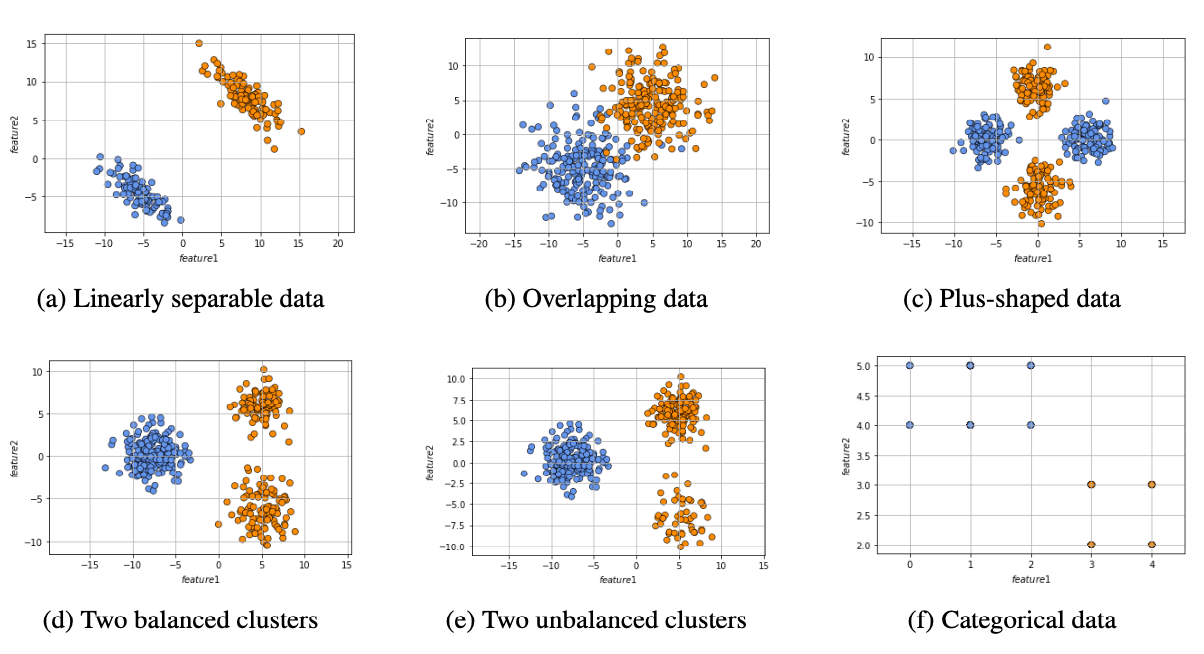
\includegraphics{www/synthetic_data.png}

}

\caption{\label{fig-synthetic-data}PLACEHOLDER: A visualization of the
synthetic classification datasets used in our experiments.}

\end{figure}

Ex-ante we expect to see that Wachter will create a new cluster of
counterfactual instances in the proximity of the initial decision
boundary. Thus, the choice of a black-box model may have an impact on
the paths of the recourse. For generators that use latent space search
(\protect\hyperlink{ref-joshi2019towards}{{[}6{]}},
\protect\hyperlink{ref-antoran2020getting}{{[}8{]}}) or rely on (and
have access to) probabilistic models
(\protect\hyperlink{ref-antoran2020getting}{{[}8{]}},
\protect\hyperlink{ref-schut2021generating}{{[}12{]}}) we expect that
counterfactuals will end up in regions of the target domain that are
densely populated by training samples. Finally, we expect to see the
counterfactuals generated by DiCE to be uniformly spread around the
feature space inside the target class.

\hypertarget{real-world-data}{%
\subsubsection{Real-world data}\label{real-world-data}}

Additionally, we use two real-world datasets from the Finance domain.
Firstly, we use the Give Me Some Credit dataset which was open-sourced
on Kaggle for the task to predict whether a borrower is likely to
experience financial difficulties in the next two years
\protect\hyperlink{ref-gmsc_data}{{[}23{]}}. Originally consisting of
250,000 instances with 11 numerical attributes, the dataset was randomly
undersampled to result in a balanced subsample made up of 3000
individuals. Secondly, we the German Credit dataset which involves the
task of predicting if bank customers are credit-worthy or not
\protect\hyperlink{ref-germancredit1994}{{[}24{]}}. It consists of 700
positive and 300 negative instances charaterized by 7 numerical and 13
categorical attributes. We process the dataset in two ways: (1) the
values of the ``Personal status and sex'' feature are aggregated by the
two represented genders; (2) the most common values are calculated for
all categorical features such that a feature \(x_d\) with the mode
\(\bar{x}_d\) is transformed into a new binary feature
\(\tilde{x}_d=\mathbb{I}_{x_{d,i}>=\bar{x}_d}\). Binarization ensures
that we can use all counterfactual generators in the benchmark.

\hypertarget{sec-method-metrics}{%
\subsection{Evaluation Metrics}\label{sec-method-metrics}}

We formulate two desiderata for the set of metrics used to measure
domain and model shifts induced by recourse. First, the metrics should
be applicable regardless of the dataset or classification technique so
that they allow for the meaningful comparison of the generators in
various scenarios. As the knowledge of the underlying probability
distribution is rarely available, the metrics should be empirical and
non-parametric. This further ensures that we can also measure large
datasets by sampling from the available data. Moreover, while our study
was conducted in a two-class classification setting, our choice of
metrics should remain applicable in the future research on multi- class
recourse problems. Second, the set of metrics should allow to capture
various aspects of the previously mentioned magnitude, path, and tempo
of changes while remaining as small as possible.

\hypertarget{domain-shifts}{%
\subsubsection{Domain Shifts}\label{domain-shifts}}

To quantify the magnitude of domain shifts we rely on an unbiased
estimate of the squared population \textbf{Maximum Mean Discrepancy
(MMD)} given as:

\begin{equation}\protect\hypertarget{eq-mmd}{}{
\begin{aligned}
MMD^2_u[F,{X}^\prime,\tilde{X}^\prime] &= \frac{1}{m(m-1)}\sum_{i=1}^m\sum_{j\neq i}^m k(x_i,x_j) \\ &+ \frac{1}{n(n-1)}\sum_{i=1}^n\sum_{j\neq i}^n k(\tilde{x}_i,\tilde{x}_j) \\ &- \frac{2}{mn}\sum_{i=1}^m\sum_{j=1}^n k(x_i,\tilde{x}_j)
\end{aligned}
}\label{eq-mmd}\end{equation}

where \(\mathcal{F}\) is a unit ball in a Reproducing Kernel Hilbert
Space H {[}27{]}, and \(X\), \(\tilde{X}\) represent independent and
identically distributed samples drawn from probability distributions
\(p\) and \(q\) respectively {[}28{]}. MMD is a measure of the distance
between the kernel mean embeddings of \(p\) and \(q\) in RKHS
\(\mathcal{H}\). An important consideration is the choice of the kernel
function \(k(\cdot,\cdot)\). In our implementation we make use of the
radial basis function (RBF) kernel with a constant length-scale
parameter of \(0.5\). As RBF captures all moments of distributions \(p\)
and \(q\), we have that \(MMD_u^2[F,X,\tilde{X}]=0\) if and only if
\(X=\tilde{X}\).

The evaluation metric in Equation~\ref{eq-mmd} is computed after every
round \(t=1,...,T\) of the experiment. To assess the statistical
significance of the observed shifts under the null hypothesis that
samples \(X\) and \(\tilde{X}\) were drawn from the same probability
distribution we follow
\protect\hyperlink{ref-arcones1992bootstrap}{{[}25{]}}. To that end, we
combine the two samples and generate a large number of permutations of
\(X + \tilde{X}\). Then, we split the permuted data into two new samples
\(X^\prime\) and \(\tilde{X}^\prime\) having the same size as the
original samples. Then under the null hypothesis we should have that
\(MMD_u^2[F,X^\prime,\tilde{X}^\prime]\) be approximately equal to
\(MMD_u^2[F,X,\tilde{X}]\). The corresponding \(p\)-value can then be
calculated by counting how these two quantities are not equal.

We calculate the MMD for both classes individually based on the ground
truth labels, i.e.~the labels that samples were assigned in time
\(t=0\). Throughout our experiments we generally do not expect the
distribution of the negative class to change over time -- application of
recourse reduces the size of this class, but since individuals are
sampled uniformly the distribution should remain unaffected. Conversely,
unless a recourse generator can perfectly replicate the original
probability distribution, we expect the MMD of the positive class to
increase. Thus, when discussing MMD, we generally mean the shift in the
distribution of the positive class.

Finally, \textbf{feature mean and feature standard deviation} are also
calculated to verify how the implementation of recourse impacts every
attribute in the dataset. Although MMD already captures information
about the expected value and variance, we may also be interested in a
more granular look at individual features.

\hypertarget{model-shifts}{%
\subsubsection{Model Shifts}\label{model-shifts}}

As our baseline for quantifying model shifts we measure perturbations to
the model parameters at each point in time \(t\) following
\protect\hyperlink{ref-upadhyay2021towards}{{[}14{]}}. We define
\(\Delta=||\theta_{t+1}-\theta_{t}||^2\), that is the euclidean distance
between the vectors of parameters before and after retraining the model
\(M\). We shall refer to this baseline metric simply as
\textbf{Perturbations}.

We extend the metric in Equation~\ref{eq-mmd} for the purpose of
quantifying model shifts. Specifically, we introduce \textbf{Predicted
Probability MMD (PP MMD)}: instead of applying Equation~\ref{eq-mmd} to
features directly, we apply it to the predicted probabilities assigned
to a set of samples by the model \(M\). If the model shifts, the
probabilities assigned to each sample will change; again, this metric
will equal 0 only if the two classifiers are the same. It is worth
noting that while we apply the technique to samples drawn uniformly from
the dataset, it can also be employed on arbitrary points in the entire
feature space (or a subspace). The latter approach is theoretically more
robust. Unfortunately, in practice this approachs suffers from the curse
of dimensionality, since it becomes increasingly difficult to select
enough points to overcome noise as the dimension \(D\) grows.

As an alternative to PP MMD we use a pseudo-distance for the
\textbf{Disagreement Coefficient} (Disagreement). This metric was
introduced in \protect\hyperlink{ref-hanneke2007bound}{{[}26{]}} and
estimates \(p(M(x) \neq M^\prime(x))\), that is the probability that two
classifiers do not agree on the predicted outcome for a randomly chosen
sample. Thus, it is not relevant whether the classification is correct
according to the ground truth, but only whether the sample lies on the
same side of the two respective decision boundaries. In our context,
this metric quantifies the overlap between the initial model (trained
before the application of recourse) and the updated model. A
Disagreement Coefficient unequal to zero is indicative of a model shift.
The opposite is not true: even if the Disagreement Coefficient is equal
to zero a model shift may still have occured. This is one reason for why
PP MMD is our our preferred metric.

Finally, we introduce \textbf{Decisiveness} as a metric that quantifies
the likelihood that a model assigns a high probability to its
classification of any given sample. We define the metric simply as
\({1\over{N}}\sum_{i=0}^N(\sigma(M(x)) − 0.5)^2\) where \(M(x)\) are
predicted logits from a binary classifier and \(\sigma\) denotes the
sigmoid function. This metric provides an unbiased estimate of the
binary classifier's tendency to produce high-confidence predictions in
either one of the two classes. Although the exact values for this metric
are not important for our study, they can be used to detect model
shifts. If decisiveness changes over time, then this is indicative of
the decision boundary moves towards either one of the two classes.

\hypertarget{sec-empirical}{%
\section{Experiments}\label{sec-empirical}}

\begin{enumerate}
\def\labelenumi{\arabic{enumi}.}
\tightlist
\item
  Shift of focus from individual to group of individuals (related:
  https://www.researchgate.net/publication/353073138\_Generating\_Collective\_Counterfactual\_Explanations\_in\_Score-Based\_Classification\_via\_Mathematical\_Optimization)
\item
  Convergence criterium matters: terminating once threshold probability
  is reached may not be optimal (see e.g.~REVISE)
\item
  Optimizer choice matters: dimensionality is typically low, so no
  obvious benefit to using ADAM.

  \begin{itemize}
  \tightlist
  \item
    This might be better placed in JuliaCon proceedings, perhaps backed
    by small blog post on the matter.
  \end{itemize}
\item
  Mitigating strategy: penaliye distance from centroid.
\end{enumerate}

\hypertarget{sec-discussion}{%
\section{Discussion}\label{sec-discussion}}

\hypertarget{sec-limit}{%
\subsection{Limitations and Future Work}\label{sec-limit}}

The experimental setup proposed here is designed to mimic a real-world
recourse process in a simple fashion. In practice, models are in fact
updated on a regular basis
\protect\hyperlink{ref-upadhyay2021towards}{{[}14{]}}. We also find it
plausible to assume that the implementation of recourse happens
periodically for different individuals, rather that all at once at time
\(t=0\). That being said, our experimental design is a vast
over-simplification of potential real-world scenarios. In practice, any
endogenous shifts that may occur can be expected to be entangled with
exogenous shifts of the nature investigated in
\protect\hyperlink{ref-upadhyay2021towards}{{[}14{]}}. We also make
implicit assumptions about the utility functions of the involved agents
that may well be too simple: individuals seeking recourse are assumed to
always implement the proposed counterfactual explanations; conversely,
the agent in charge of the model \(M\) is assumed to always treat
individuals that have implemented valid recourse as if they were truly
now in the target class. Relating this back to the consumer credit
example, we assume that the would-be borrowers are always willing and
able to implement recourse and the bank is always willing to provide
credit as would-be borrowers move across the decision boundary. In
practice it is doubtful that agents behave according to such simple
rules. Nonetheless, we think that our simple framework offers a starting
point for future work on recourse dynamics (both endogenous and
exogenous dynamics).

\hypertarget{data}{%
\subsubsection{Data}\label{data}}

The number of real-world datasets considered in this work is limited,
constrained by the fact that at the time of writing
\texttt{CounterfactualExplanations.jl} only supported continuous
features.

\hypertarget{sec-conclusion}{%
\section{Concluding Remarks}\label{sec-conclusion}}

\hypertarget{acknowledgment}{%
\section*{Acknowledgment}\label{acknowledgment}}
\addcontentsline{toc}{section}{Acknowledgment}

P. A. thanks \ldots{}

\pagebreak
\FloatBarrier

\hypertarget{references}{%
\section*{References}\label{references}}
\addcontentsline{toc}{section}{References}

\hypertarget{refs}{}
\begin{CSLReferences}{0}{0}
\leavevmode\vadjust pre{\hypertarget{ref-borch2022machine}{}}%
\CSLLeftMargin{{[}1{]} }%
\CSLRightInline{C. Borch, {``Machine learning, knowledge risk, and
principal-agent problems in automated trading,''} \emph{Technology in
Society}, p. 101852, 2022.}

\leavevmode\vadjust pre{\hypertarget{ref-o2016weapons}{}}%
\CSLLeftMargin{{[}2{]} }%
\CSLRightInline{C. O'neil, \emph{Weapons of math destruction: How big
data increases inequality and threatens democracy}. Crown, 2016.}

\leavevmode\vadjust pre{\hypertarget{ref-rudin2019stop}{}}%
\CSLLeftMargin{{[}3{]} }%
\CSLRightInline{C. Rudin, {``Stop explaining black box machine learning
models for high stakes decisions and use interpretable models
instead,''} \emph{Nature Machine Intelligence}, vol. 1, no. 5, pp.
206--215, 2019.}

\leavevmode\vadjust pre{\hypertarget{ref-pawelczyk2021carla}{}}%
\CSLLeftMargin{{[}4{]} }%
\CSLRightInline{M. Pawelczyk, S. Bielawski, J. van den Heuvel, T.
Richter, and G. Kasneci, {``Carla: A python library to benchmark
algorithmic recourse and counterfactual explanation algorithms,''}
\emph{arXiv preprint arXiv:2108.00783}, 2021.}

\leavevmode\vadjust pre{\hypertarget{ref-wachter2017counterfactual}{}}%
\CSLLeftMargin{{[}5{]} }%
\CSLRightInline{S. Wachter, B. Mittelstadt, and C. Russell,
{``Counterfactual explanations without opening the black box: Automated
decisions and the GDPR,''} \emph{Harv. JL \& Tech.}, vol. 31, p. 841,
2017.}

\leavevmode\vadjust pre{\hypertarget{ref-joshi2019towards}{}}%
\CSLLeftMargin{{[}6{]} }%
\CSLRightInline{S. Joshi, O. Koyejo, W. Vijitbenjaronk, B. Kim, and J.
Ghosh, {``Towards realistic individual recourse and actionable
explanations in black-box decision making systems,''} \emph{arXiv
preprint arXiv:1907.09615}, 2019.}

\leavevmode\vadjust pre{\hypertarget{ref-mothilal2020explaining}{}}%
\CSLLeftMargin{{[}7{]} }%
\CSLRightInline{R. K. Mothilal, A. Sharma, and C. Tan, {``Explaining
machine learning classifiers through diverse counterfactual
explanations,''} in \emph{Proceedings of the 2020 conference on
fairness, accountability, and transparency}, 2020, pp. 607--617.}

\leavevmode\vadjust pre{\hypertarget{ref-antoran2020getting}{}}%
\CSLLeftMargin{{[}8{]} }%
\CSLRightInline{J. Antorán, U. Bhatt, T. Adel, A. Weller, and J. M.
Hernández-Lobato, {``Getting a clue: A method for explaining uncertainty
estimates,''} \emph{arXiv preprint arXiv:2006.06848}, 2020.}

\leavevmode\vadjust pre{\hypertarget{ref-karimi2020survey}{}}%
\CSLLeftMargin{{[}9{]} }%
\CSLRightInline{A.-H. Karimi, G. Barthe, B. Schölkopf, and I. Valera,
{``A survey of algorithmic recourse: Definitions, formulations,
solutions, and prospects,''} \emph{arXiv preprint arXiv:2010.04050},
2020.}

\leavevmode\vadjust pre{\hypertarget{ref-verma2020counterfactual}{}}%
\CSLLeftMargin{{[}10{]} }%
\CSLRightInline{S. Verma, J. Dickerson, and K. Hines, {``Counterfactual
explanations for machine learning: A review,''} \emph{arXiv preprint
arXiv:2010.10596}, 2020.}

\leavevmode\vadjust pre{\hypertarget{ref-ustun2019actionable}{}}%
\CSLLeftMargin{{[}11{]} }%
\CSLRightInline{B. Ustun, A. Spangher, and Y. Liu, {``Actionable
recourse in linear classification,''} in \emph{Proceedings of the
conference on fairness, accountability, and transparency}, 2019, pp.
10--19.}

\leavevmode\vadjust pre{\hypertarget{ref-schut2021generating}{}}%
\CSLLeftMargin{{[}12{]} }%
\CSLRightInline{L. Schut \emph{et al.}, {``Generating interpretable
counterfactual explanations by implicit minimisation of epistemic and
aleatoric uncertainties,''} in \emph{International conference on
artificial intelligence and statistics}, 2021, pp. 1756--1764.}

\leavevmode\vadjust pre{\hypertarget{ref-karimi2021algorithmic}{}}%
\CSLLeftMargin{{[}13{]} }%
\CSLRightInline{A.-H. Karimi, B. Schölkopf, and I. Valera,
{``Algorithmic recourse: From counterfactual explanations to
interventions,''} in \emph{Proceedings of the 2021 ACM conference on
fairness, accountability, and transparency}, 2021, pp. 353--362.}

\leavevmode\vadjust pre{\hypertarget{ref-upadhyay2021towards}{}}%
\CSLLeftMargin{{[}14{]} }%
\CSLRightInline{S. Upadhyay, S. Joshi, and H. Lakkaraju, {``Towards
robust and reliable algorithmic recourse,''} \emph{arXiv preprint
arXiv:2102.13620}, 2021.}

\leavevmode\vadjust pre{\hypertarget{ref-rabanser2019failing}{}}%
\CSLLeftMargin{{[}15{]} }%
\CSLRightInline{S. Rabanser, S. Günnemann, and Z. Lipton, {``Failing
loudly: An empirical study of methods for detecting dataset shift,''}
\emph{Advances in Neural Information Processing Systems}, vol. 32,
2019.}

\leavevmode\vadjust pre{\hypertarget{ref-chandola2009anomaly}{}}%
\CSLLeftMargin{{[}16{]} }%
\CSLRightInline{V. Chandola, A. Banerjee, and V. Kumar, {``Anomaly
detection: A survey,''} \emph{ACM computing surveys (CSUR)}, vol. 41,
no. 3, pp. 1--58, 2009.}

\leavevmode\vadjust pre{\hypertarget{ref-widmer1996learning}{}}%
\CSLLeftMargin{{[}17{]} }%
\CSLRightInline{G. Widmer and M. Kubat, {``Learning in the presence of
concept drift and hidden contexts,''} \emph{Machine learning}, vol. 23,
no. 1, pp. 69--101, 1996.}

\leavevmode\vadjust pre{\hypertarget{ref-gama2014survey}{}}%
\CSLLeftMargin{{[}18{]} }%
\CSLRightInline{J. Gama, I. Žliobaitė, A. Bifet, M. Pechenizkiy, and A.
Bouchachia, {``A survey on concept drift adaptation,''} \emph{ACM
computing surveys (CSUR)}, vol. 46, no. 4, pp. 1--37, 2014.}

\leavevmode\vadjust pre{\hypertarget{ref-nelson2015evaluating}{}}%
\CSLLeftMargin{{[}19{]} }%
\CSLRightInline{K. Nelson, G. Corbin, M. Anania, M. Kovacs, J. Tobias,
and M. Blowers, {``Evaluating model drift in machine learning
algorithms,''} in \emph{2015 IEEE symposium on computational
intelligence for security and defense applications (CISDA)}, 2015, pp.
1--8.}

\leavevmode\vadjust pre{\hypertarget{ref-ackerman2021machine}{}}%
\CSLLeftMargin{{[}20{]} }%
\CSLRightInline{S. Ackerman, P. Dube, E. Farchi, O. Raz, and M.
Zalmanovici, {``Machine learning model drift detection via weak data
slices,''} in \emph{2021 IEEE/ACM third international workshop on deep
learning for testing and testing for deep learning (DeepTest)}, 2021,
pp. 1--8.}

\leavevmode\vadjust pre{\hypertarget{ref-de2021framework}{}}%
\CSLLeftMargin{{[}21{]} }%
\CSLRightInline{R. M. B. de Oliveira and D. Martens, {``A framework and
benchmarking study for counterfactual generating methods on tabular
data,''} \emph{Applied Sciences}, vol. 11, no. 16, p. 7274, 2021.}

\leavevmode\vadjust pre{\hypertarget{ref-altmeyer2022CounterfactualExplanations}{}}%
\CSLLeftMargin{{[}22{]} }%
\CSLRightInline{P. Altmeyer, \emph{{CounterfactualExplanations.jl - a
Julia package for Counterfactual Explanations and Algorithmic
Recourse}}. 2022. Available:
\url{https://github.com/pat-alt/CounterfactualExplanations.jl}}

\leavevmode\vadjust pre{\hypertarget{ref-gmsc_data}{}}%
\CSLLeftMargin{{[}23{]} }%
\CSLRightInline{K. Competition, {``Give me some credit, improve on the
state of the art in credit scoring by predicting the probability that
somebody will experience financial distress in the next two years.''}
\url{https://www.kaggle.com/c/GiveMeSomeCredit}}

\leavevmode\vadjust pre{\hypertarget{ref-germancredit1994}{}}%
\CSLLeftMargin{{[}24{]} }%
\CSLRightInline{H. Hoffman, {``German credit data,''} 1994.
\url{https://archive.ics.uci.edu/ml/datasets/statlog+(german+credit+data)}}

\leavevmode\vadjust pre{\hypertarget{ref-arcones1992bootstrap}{}}%
\CSLLeftMargin{{[}25{]} }%
\CSLRightInline{M. A. Arcones and E. Gine, {``On the bootstrap of u and
v statistics,''} \emph{The Annals of Statistics}, pp. 655--674, 1992.}

\leavevmode\vadjust pre{\hypertarget{ref-hanneke2007bound}{}}%
\CSLLeftMargin{{[}26{]} }%
\CSLRightInline{S. Hanneke, {``A bound on the label complexity of
agnostic active learning,''} in \emph{Proceedings of the 24th
international conference on machine learning}, 2007, pp. 353--360.}

\end{CSLReferences}

\pagebreak

\hypertarget{tables}{%
\section{Tables}\label{tables}}

\ldots{}

\pagebreak

\hypertarget{figures}{%
\section{Figures}\label{figures}}

\ldots{}

\pagebreak

\hypertarget{code}{%
\section{Code}\label{code}}

\ldots{}



\end{document}
